\chapter{Communication protocol}\label{chap:comm}
For the main hardware components to be able to communicate, some kind of network communication has to be defined. Throughout this chapter the communication hardware, methods and final design of this network will be introduced.

\nomenclature{SPI}{Serial Peripheral Interface}

\section{Low level protocol specification}
In \marginnote{Not sure about the exact placement of each part of section. Let's talk about that some day!}[-25pt] the assignment proposal it is given that the communication interface between the FPGA and LM3S6965 microcontroller must be SPI. There are no formal SPI protocol standards however, so it must be decided how the link will work. The Stellaris SSI\footnote{Synchronous Serial Interface} module supports three different interfaces: Freescale SPI, MICROWIRE and Texas Instruments SSI. The main difference between these three formats is how they handle each individual serial frame.

The Freescale SPI mode of operation is chosen, as it enables full-duplex transmission (which MICROWIRE does not) and because of the way the select signal (\texttt{SSIFss}) works in this mode. Using the Freescale frame format, the \texttt{SSIFss} is high while the communication line is idle. \marginnote{This calls for an illustration} It is then pulled low while sending a frame. Pulling it low thus signifies the beginning of a frame, and pulling it high tells the slave that the frame is at its end. The Texas Instruments SSI format works by instead pulsing its \texttt{SSIFss} signal for only one \texttt{SSIClk} period to signify the beginning and ending of a frame. This is deemed more error prone as there is no time in-between frames to synchronize. Freescale SPI has one \texttt{SSIClk} period in-between frames, where \texttt{SSIFss} gets pulled high, allowing the slave a chance to "catch up".\nomenclature{SSI}{Synchronous Serial Interface}

The LM3S6965 microcontroller will be operating as master and the FPGA as slave, letting the microcontroller when communication should take place.

%------------------------------------------
\section{SPI introduction}
SPI is short for Serial Peripheral Interface, and is a commonly used standard for internal communication between hardware. Because SPI is a commonly used transmission interface, this will only contain a short introduction. The \marginnote{Check me}{simplest} SPI connection consists of a master, a slave and 4 signal lines: A clock, a signal from master to slave (MOSI\footnote{Master Out Slave In}), a signal from slave to master (MISO\footnote{Master In Slave Out}) and a slave select (SS) signal. The clock is used to control when to put data on the signal lines, and is always controlled by the master device. This way the master device always controls when there is data available on the signal lines, and at what data rate the it is send. An effect of this is that, for the master to be able to get a reply from the slave, some extra data needs to be send to activate the data carrying clock. The synchronisation between the clock and the data on the MOSI and MISO lines can be set up in four different ways, depending on the clock phase (CPHA) and polarity (CPOL). The slave select signal is used to enable the transmission on the slave device. When pulled low, the slave device starts listening for data from the master device. This enables the use of the clock, MOSI and MISO lines for multiple devices. 
% What is SPI
% Limitations

%CPOL CPHA

% SPI stands for Serial Peripheral Interface
% Used for moving data simply and quickly from one device to another
% Serial Interface
% Synchronous
% Master-Slave
% Data Exchange
% Data on SCK  (the clock rate can vary, unlike RS-232 style communications)
% SPI sync modes
% WIKI fact:  frequencies are commonly in the range of 1�70 MHz

%\subsection{Hardware support}
% Support on ARM development board -- The LM3S6965 controller includes one SSI module that provides the functionality for synchronous
% serial communications with peripheral devices, and can be configured to use the Freescale SPI,
% MICROWIRE, or TI synchronous serial interface frame formats. The size of the data frame is also
% configurable, and can be set between 4 and 16 bits, inclusive.

% Separate transmit and receive FIFOs, 16 bits wide, 8 locations deep

%\subsection{Inspiration for protocol}
% ArcNet / PA10
% CAN / DeviceNet
% ADNS9500 Mouse sensor, IMU sensor
% - What is it used for, and why is it interesting to look at?
%The first approach for designing the SPI protocol was to look for  
\section{Protocol requirements}
Selection the right protocol design for a project greatly depends on the requirements from the other parts as the system. Such requirements would include: 
\begin{itemize}
\item Noise on transmission lines (Need for error correction or detection)
\item Security (encryption)
\item Package synchronisation (Start and stop flags)
\item The size of data to be transmitted (Minimum transmission speed)
\item Timing criteria (Do we need to know how old the data are)
\end{itemize}

Because the data only needs to travel a short distance, noise and security is not considered as a problem in this project. Even if noise should occur, a lot of things could be done to the physical parts to solve this without involving redesign of the protocol (Ex. paired and shielded cables). 
The protocol are using SPI, so there is no need for synchronising the packages, as this can be done by the SS signal line. This eliminates the needs for overhead such as start or stop flags on packages. 
\marginnote{Read and comment if it's good enough}The ARM runs the SPI connection at a speed of 1MHz. Each clock pulse transmits 1bit, so 2MHz will carry 2Mbps = 256KBps. With this transmission rate, it will be possible to read or write an entire 32byte memory block at a rate of $\frac{32B}{256KBps} \approx 8KHz$. The ARM is capable of running the SPI at much greater speeds then 2MHz, and a update rate of 8KHz is a lot more then needed, considered physical speed limitations of the \marginnote{pan/tilt}{pan/tilt} system.


\section{Protocol ideas}
\label{spi_protocol_ideas}
During the design of the protocol three approaches were considered. These three approaches and the final protocol solution are described below.


\subsection{Specialised protocol}
The first approach was to design the protocol to carry just the information that needs to be exchanged between the FPGA and ARM boards. A data package would then consist of a header followed by a series of only the needed data. This idea had the advantage of a low overhead on the protocol and thereby a minimal need for resources on the platforms. This idea was discarded, because a change in the data requirements would require a redesign of the protocol.

\subsection{Memory synchronisation protocol}
Another approach to the protocol design was to make a protocol to synchronise a static sized memory between the two platforms. The idea was to take advantage of the 16bit x 8 FIFO on the ARM platform, so one package would fit exactly into it. The advantage would be that the ARM processor only needs to be interrupted when the FIFO was full. A similar solution would then be written in hardware to the FPGA, making this solution quite efficient. The large amount of data in one package would allow a CRC or checksum to be implemented without too much overhead. An example of how this protocol could be made is shown in figure \ref{fig:spi_protocol_format_memsync}.

\begin{figure}[htb]
	\centering
	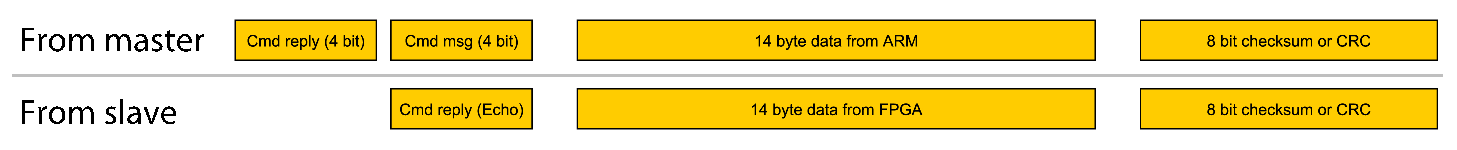
\includegraphics[width=0.96\textwidth,trim=0 0 0 0]{graphics/spi_protocol_format_memsync.pdf} %trim=l b r t (can cut off from every side)
	\caption{An example of the protocol design with the memory synchronisation protocol approach}
	\label{fig:spi_protocol_format_memsync}			% figure labels are of the form 
\end{figure}

The first four bits from the master decides what the slave shall respond. The next four bits describes what the master is sending to the slave. After the slave has received the first four bits, it immediately echoes the command followed by the requested data.

\subsection{Generic protocol}
\label{spi_generic_protocol}
The generic approach was to make the protocol compatible with the protocol of other SPI devices. Because a lot of SPI devices uses specialised protocols, there is not a generic approach as such. Some devices tough share a way of reading and writing registers on the hardware, which in this document will be referred as a generic way. Using this protocol will give the great advantage of both reusable code/hardware, fairly easy implementation and good scalability. The generic design approach was chosen as most appropriate solution for this project and will be described in greater details in section \ref{spi_rotocol_design}.


%\section{Protocol selection discussion}
%Something that sounds smart or REMOVE ME.

%The ADNS9500 mouse sensor and ADIS16405 IMU sensor SPI interface protocols were used as reference designs, as these are well known form earlier projects.  

% Burst mode
% i2c
% error correction / detection
% Error detection
% Room for extending protocol

\section{Protocol design}
\label{spi_rotocol_design}
It has been decided to use a generic\footnote{See \ref{spi_generic_protocol} for a definition of generic} way of communicating with SPI between the FPGA and ARM board. Other ideas were considered and can be read about in \ref{spi_protocol_ideas}.
The main advantage for choosing a generic design is the simple implementation and compatibility with other SPI devices. The ADNS9500~\cite{SPI_ADNS} mouse sensor and the ADIS16405~\cite{SPI_ADIS} IMU sensor were used as protocol reference devices, as these has been used in previous projects. The main difference between the protocol in these two devices are the length of the carried data. The ADNS9500 reads and writes only 8 bits at a time, where ADIS16405 supports 16bit data sizes. The 8 bit solution was chosen as reference.

For synchronisation of clock and data on the signal lines, mode 0 was chosen. Mode 0 is when data is available on clock rising edge and changes on falling edge.

% Depending on the address it can be read only, write only or read/write. 
The general idea is that the SPI slave has a memory block, which the SPI master can read and write from. The list of addresses are determined by the hardware modules on the FGPA and can be found in table \ref{tab:Memorymapping}. The protocol itself is pretty straight forward. The MSB determines if it is a read or write operation, and the last 5 bits determines the address or function. The two bits in between are reserved for future use, and should always be set to zero. The five address bits in the current design gives access to 32 bytes of memory on the slave device, which is enough to hold the data for this project. The command structure is shown in figure \ref{fig:spi_protocol_cmd_structure}. Both reference devices supports a burst command, where a series of relevant data are sent as response of a single command. There was no need to implement such functionality in this design. How the reading and writing is done is described below.
\begin{figure}[htb]
	\centering
	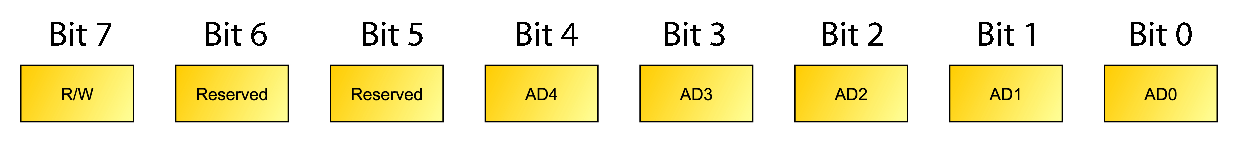
\includegraphics[width=0.96\textwidth,trim=0 0 0 0]{graphics/spi_protocol_cmd_structure.pdf} %trim=l b r t (can cut off from every side)
	\caption{Bit structure of the SPI command send from master to slave}
	\label{fig:spi_protocol_cmd_structure}			% figure labels are of the form 
\end{figure}


\subsection{Reading from slave device}
When the master needs to read from the slave device it sends a byte with the MSB\footnote{Most significant bit} to low, and the last five bits according to the address to be read. Meanwhile the command is send, the slave may be sending the response from last command, or just zeroes if it has nothing to return. For the master to be able to receive the response, it needs to send a byte because SPI is synchronous. This may be the next command or just zeroes. The reason for this is, that the communication is always initiated from the master device on SPI. A read command sequence is shown in figure \ref{fig:spi_protocol_command_structure_read} 

\begin{figure}[htb]
	\centering
	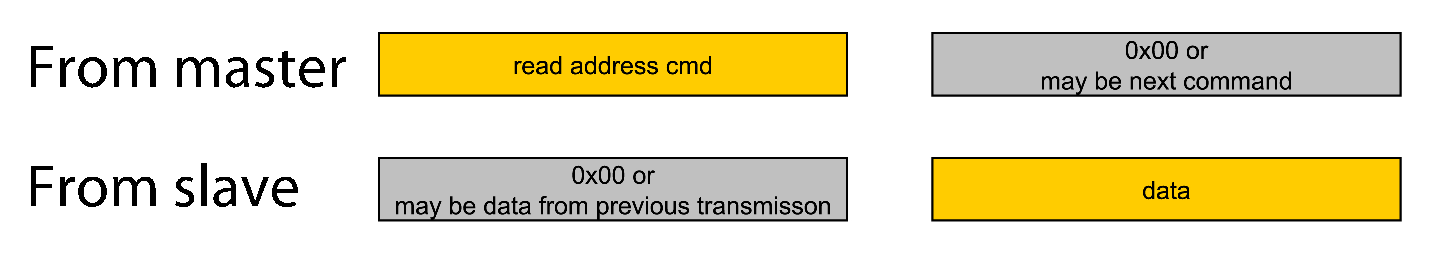
\includegraphics[width=0.96\textwidth]{graphics/spi_protocol_command_structure_read_wlabels.pdf} %trim=l b r t (can cut off from every side)
	\caption{SPI communication when reading from the slave}
	\label{fig:spi_protocol_command_structure_read}			% figure labels are of the form \label{fig:*}
\end{figure}


\subsection{Writing to slave device}
The command send from the master device when writing to the slave device is similar to the one used to read the same address, but with the MSB set to high. The structure of the command byte is shown in figure \ref{fig:spi_protocol_cmd_structure}. Meanwhile the command is send, the slave may be sending the response from last command, or just zeroes if it has nothing to return. Next the master sends the value to be written to the address from the command byte. While the value is send, the output from the slave is just an empty byte. The write sequence is shown in figure \ref{fig:spi_protocol_command_structure_write}.

\begin{figure}[htb]
	\centering
	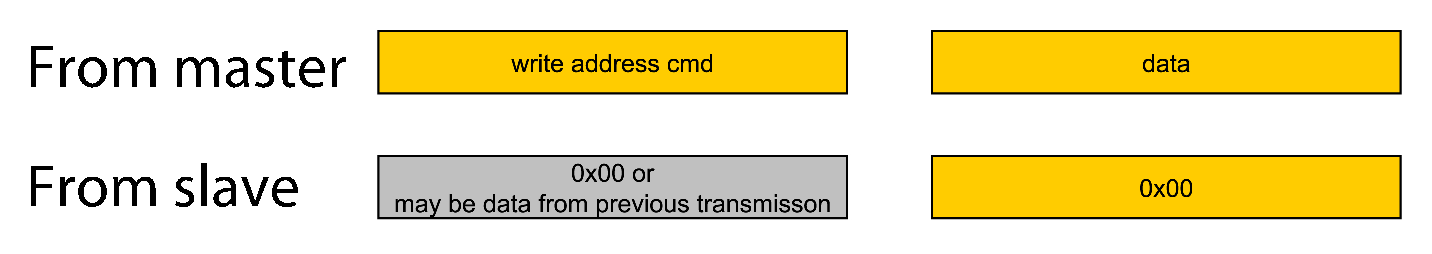
\includegraphics[width=0.96\textwidth]{graphics/spi_protocol_command_structure_write_wlabels.pdf} %trim=l b r t (can cut off from every side)
	\caption{SPI communication when writing to the slave}
	\label{fig:spi_protocol_command_structure_write}			% figure labels are of the form \label{fig:*}
\end{figure}



\section{Protocol ARM implementation}
%\section{Protocol ARM implementation}
One integral part of the project is the communication between the microprocessor and FPGA devices. This section describes the process of implementing SPI communication software (in the remainder of this section just referred to as the \textit{implementation}) on the microprocessor. It will go over the initial demands of the implementation, how it was made, how it works, and how it is supposed to be used (by other parts of the system). A test of the implementation is also described. Finally, the results the test yielded, plus thoughts about further improvements, are discussed.

\subsection{Requirements and delimitations}\label{sec:spi_software_reqs}
The first part of the development process was to specify requirements to the implementation, to make it easier for the rest of the software system to make use of the SPI link. Those requirements were:
\begin{enumerate}
  \item The implementation would have to be multi-task/thread safe, as more than one task may have to use the SPI software interface at any given time.
  \item The interface provided by the implementation should be easy to use by other processes in the system.
\end{enumerate}

To fulfill the first requirement, some problems has to be considered carefully: If more than one task uses the implementations interface to send data asynchronously, how do they receive data back in the correct order? There is only one physical SPI link in the LM3S6965, so it has to be handled by software.
The microcontroller is the exclusive \textit{master} of the SPI link, so only it can initiate communication. The software relies heavily on that fact to facilitate multi-task usage. Also, every time a unit data is sent, the same amount will be received. That way we know, that if a task sends data, the data which is returned immediately afterwards should be directed to that particular task.

The second requirement states that an easy-to-use interface should be provided - in practice through the modules header-file. What is meant with that is, that the user-task should not have to worry about whether or not it is allowed to write to the SPI hardware FIFO at the time it makes a call to the implementation. Additionally, when a task is reading return-data, it should not have to worry about whether it is correctly reading data meant for it, or reading data meant for another task.

Since the whole embedded software system is based on the FreeRTOS real-time kernel, most of the constructs used to implement the SPI communication software, like semaphores and queues, are those provided by the FreeRTOS API.

The documentation of the implementation is split into two parts: One being the interface - the link to the ``outside world'' - and one being the actual transmission and reception to or from the hardware layer FIFO buffers.



\subsection{Interface}
The topmost layer of the implementation is the interface between the SPI implementation and the rest of the program.

The interface quite simply consists of the four functions \texttt{spi\_init}, \texttt{spi\_register\_task}, \texttt{spi\_write\_from\_task} and \texttt{spi\_read\_from\_task}. The \texttt{\_task}-suffix signifies that the function is meant to be called from within a task (and will otherwise have no effect).

The first function to be called under normal circumstances would be \texttt{spi\_init}. It initializes the hardware SPI peripheral for use such as described in [ref freescale etc.]. Also, it creates two tasks; a transmitter and a receiver as well as associated queues and semaphores.

\begin{figure}[htb]
  \begin{subfigure}[b]{0.495\textwidth}
    \centering
    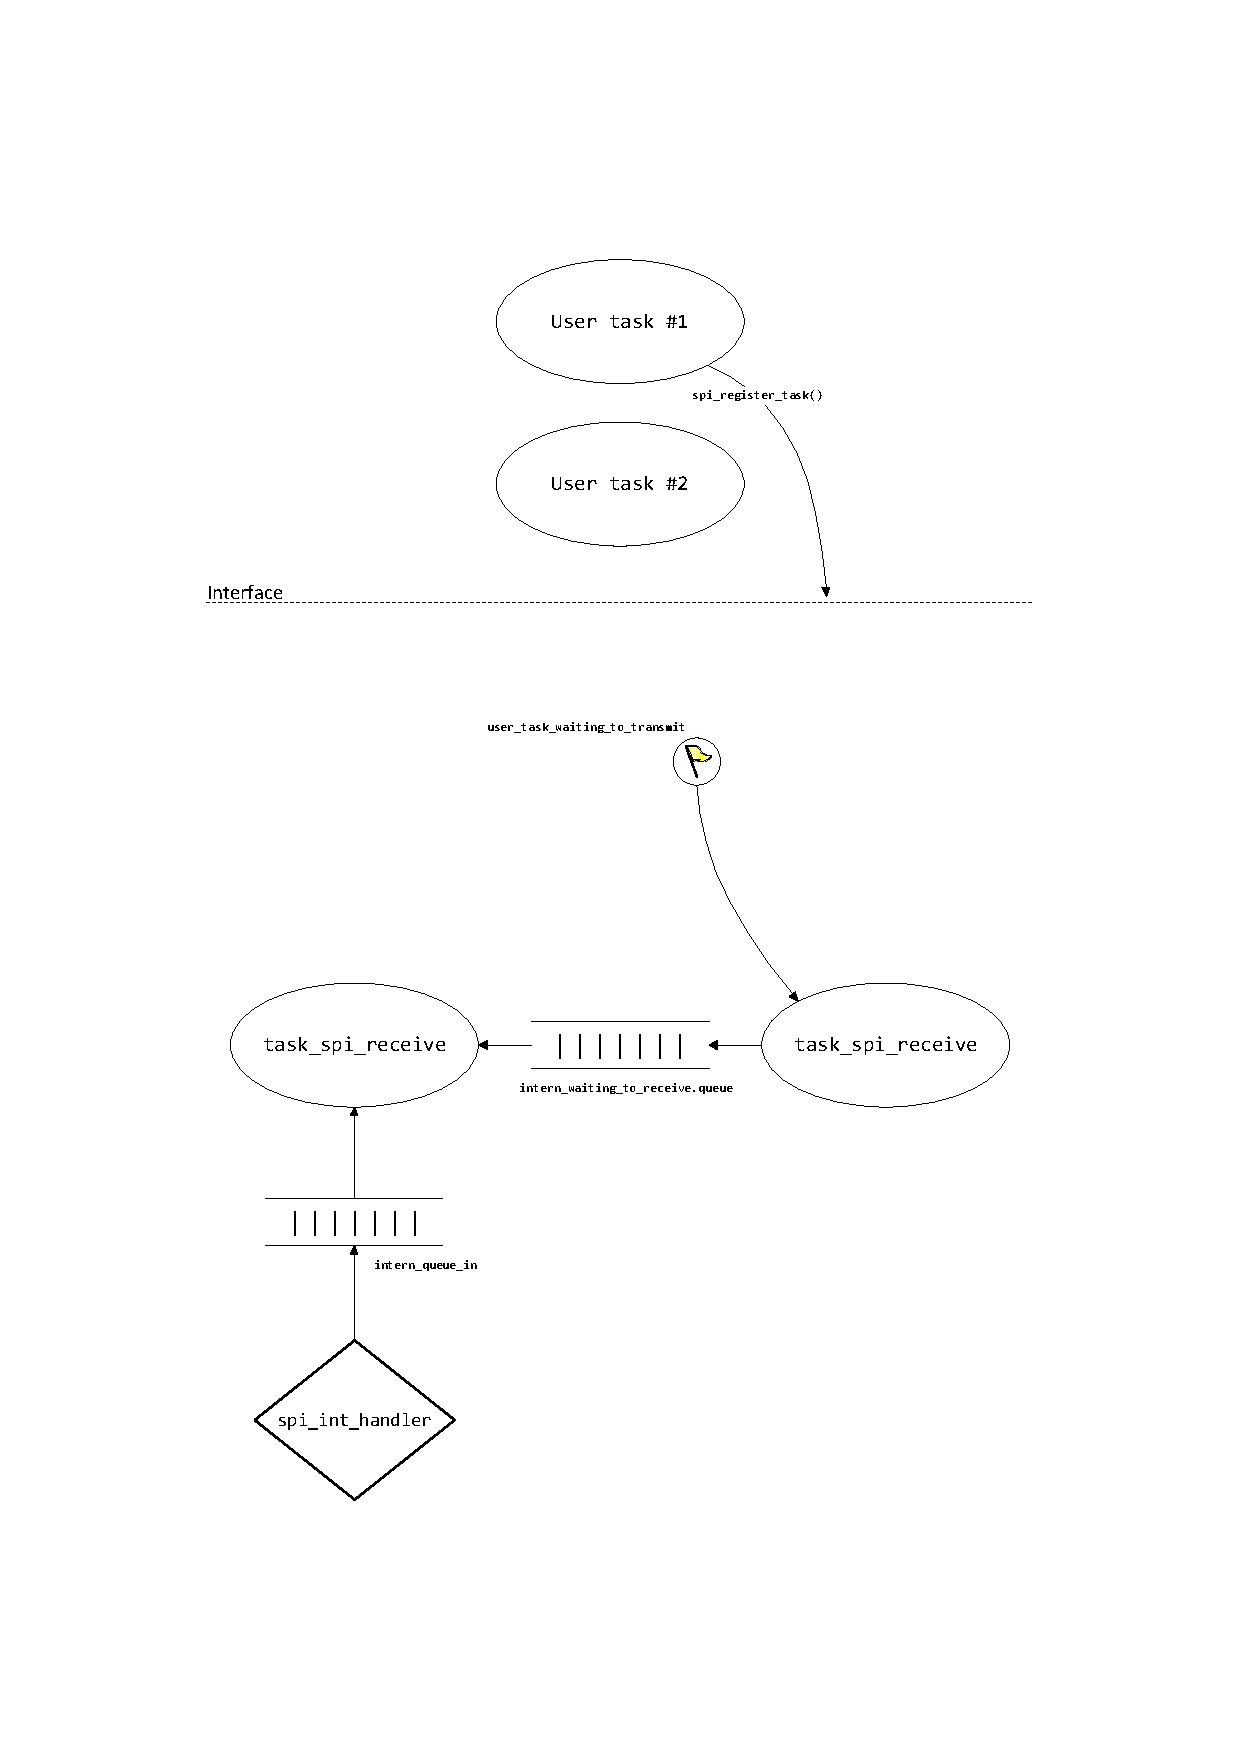
\includegraphics[width=\textwidth,clip,trim=0 0 0 0]{content/04_communication/figures/spi_task_diagram_initial_1.pdf}
    \caption{Before the \texttt{spi\_register\_task} call.}
    \label{fig:spi_task_diagram_initial_1}
  \end{subfigure}
  \begin{subfigure}[b]{0.495\textwidth}
    \centering
    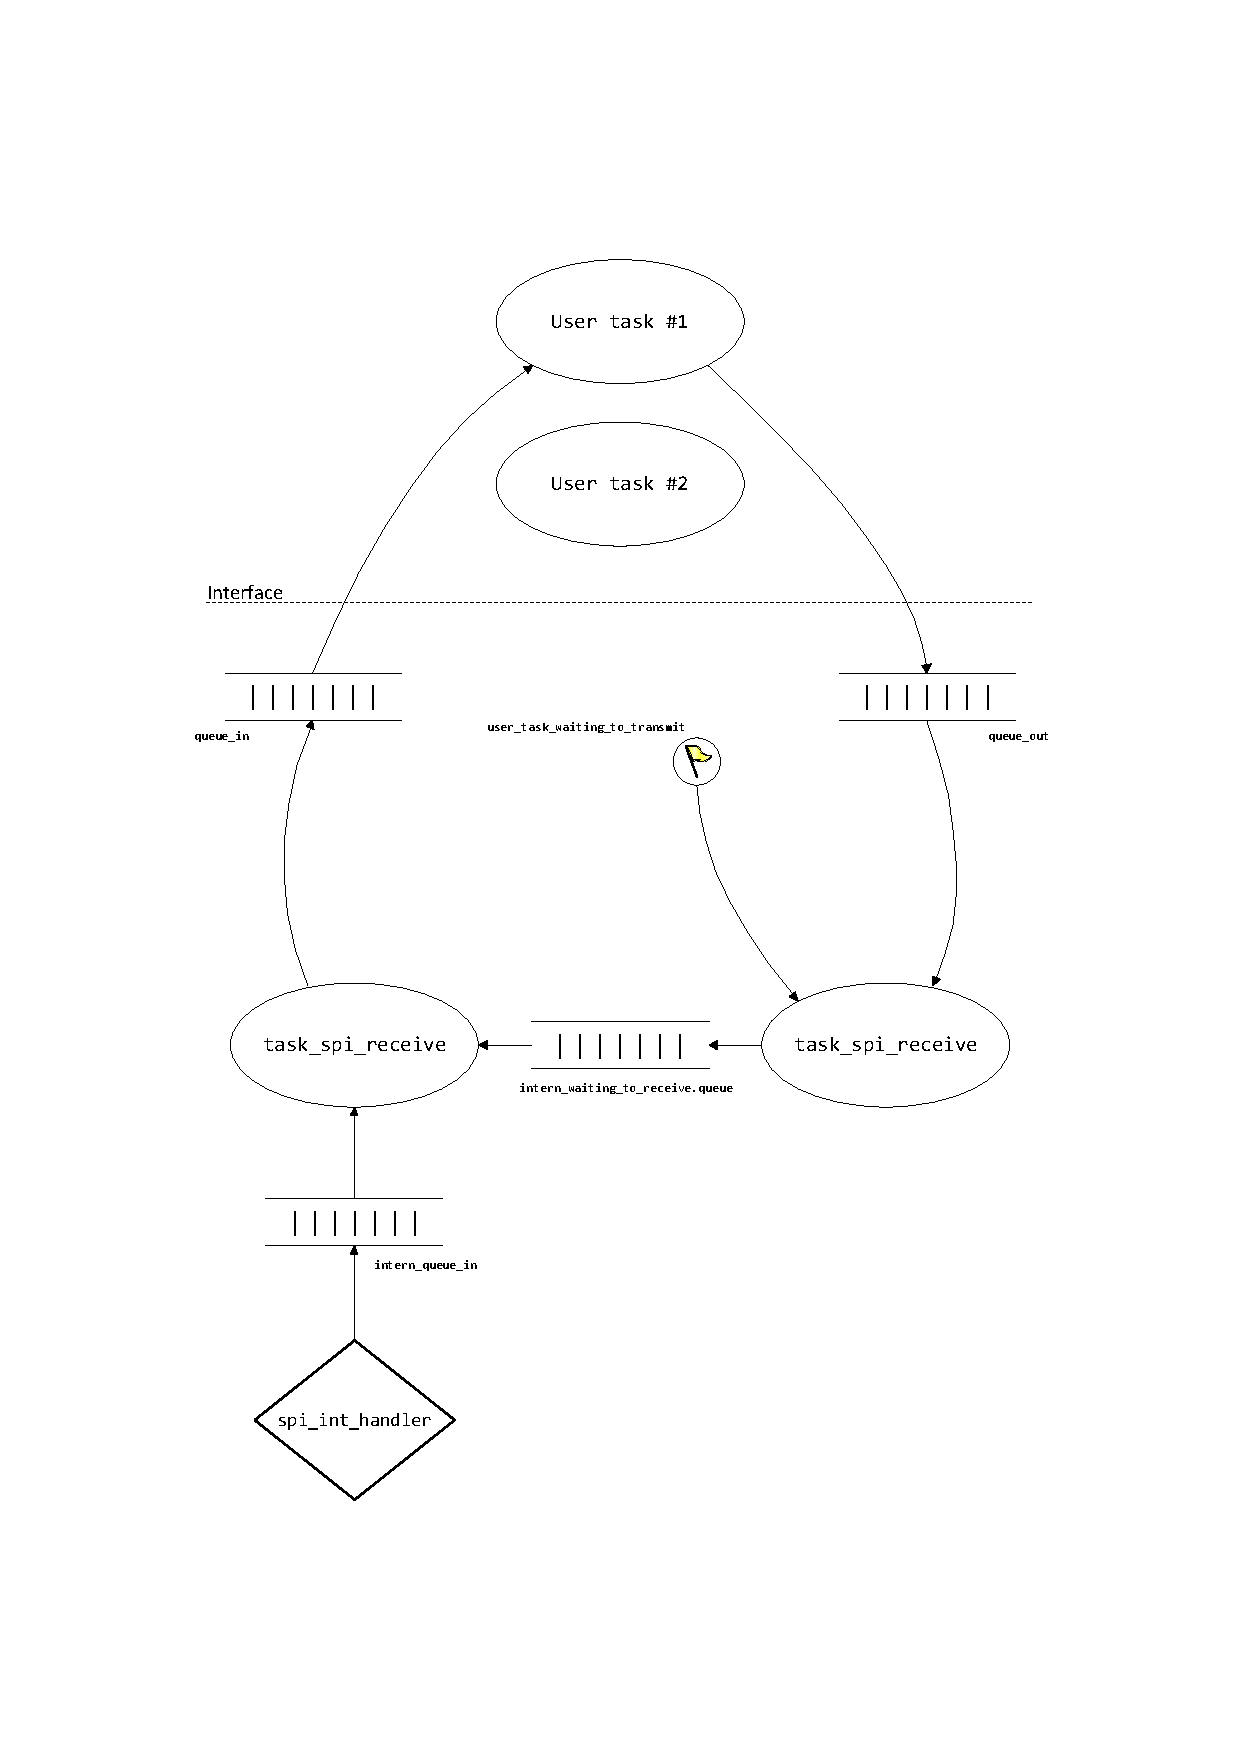
\includegraphics[width=\textwidth,clip,trim=0 0 0 0]{content/04_communication/figures/spi_task_diagram_initial_2.pdf}
    \caption{After the \texttt{spi\_register\_task} call.}
    \label{fig:spi_task_diagram_initial_2}
  \end{subfigure}
  \caption{A user task registering with the SPI interface.}
  \label{fig:spi_register_task}
\end{figure}%trim=l b r t

For at task to be able to use the SPI link, it will have to first make a call to the function \texttt{spi\_register\_task}. That is because resources are allocated dynamically (described in \ref{sec:spi_underthehood}.). Figure \ref{fig:spi_register_task} shows a user task using the register function and getting queues allocated to it. 

When a user task has been successfully registered with the SPI software it is allowed use of the \texttt{spi\_write\_from\_task}- and \texttt{spi\_read\_from\_task}-functions to read and write to and from its private queues. With only those two functions used frequently during runtime, the second design goal is considered fulfilled.

An overview - a task diagram - is shown in figure \ref{fig:spi_task_diagram}.



\subsection{Under the hood}\label{sec:spi_underthehood}
To understand how the implementation works, lets describe what goes on ``under the hood''. That is, between the user interface and the hardware transmit/receive logic. The first design goal was, that the implementation should be thread-safe. To elaborate; the implementation should allow multiple tasks to send and receive data asynchronously. To make that possible, a scheme, where each task gets its own private software buffers for transmission and reception, is used. That way the software implementation can imitate multiple SPI hardware interfaces. The implementation works is such a way that these ``private'' queues are allocated dynamically when a task wishes to use the SPI. The task which wishes to use the SPI is then associated with the queues by task handle.\footnote{A way of uniquely identifying tasks provided by the FreeRTOS API.} The private queues can be seen just below the ``interface line'' on the task diagram in figure \ref{fig:spi_task_diagram}.

\begin{figure}[htb]
  \centering
  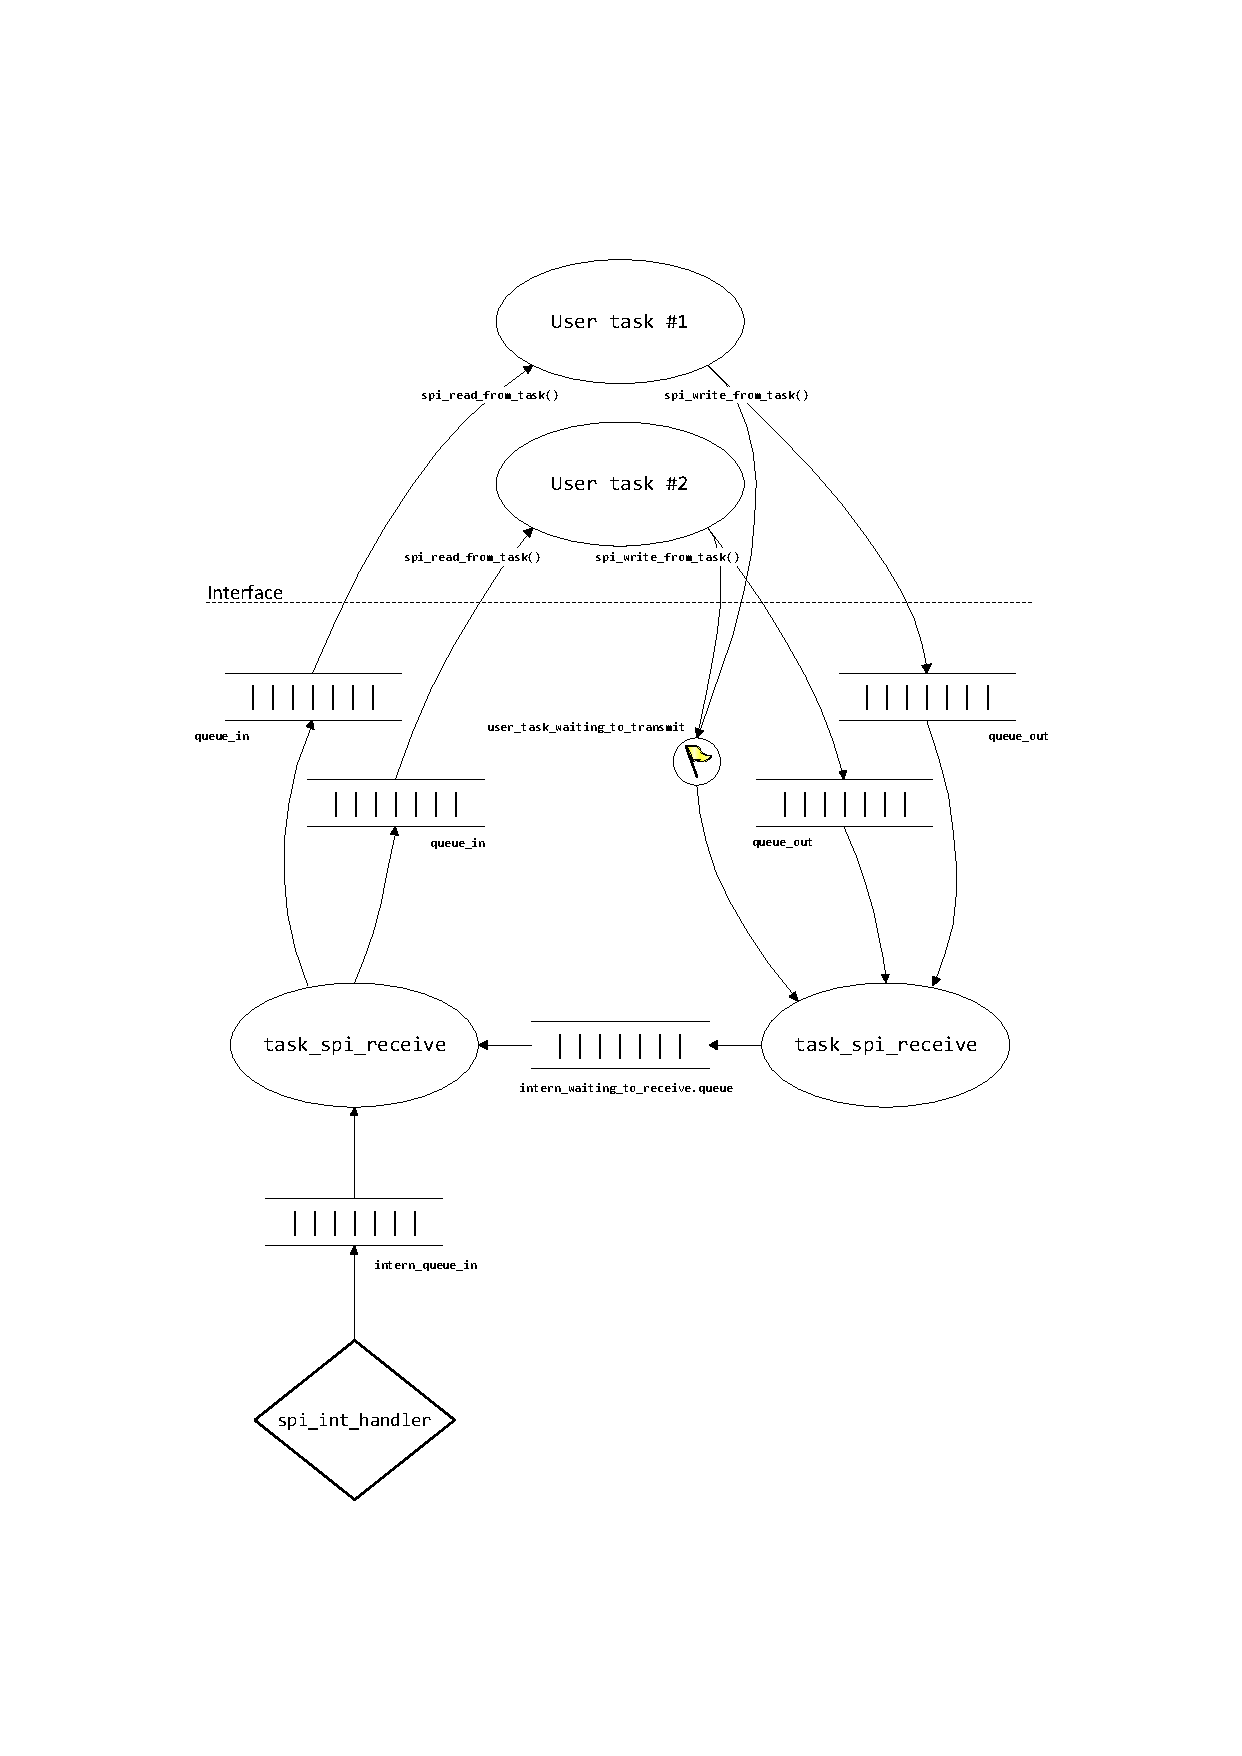
\includegraphics[width=\textwidth,clip,trim=0 15 0 15]{content/04_communication/figures/spi_task_diagram_running.pdf}
  \caption{An overview of the SPI implementation.}
  \label{fig:spi_task_diagram}
\end{figure}%trim=l b r t

A doubly linked list is used to keep track of tasks using the SPI implementation. Each element in the list is a variable that contain the handle of the user task, associated queues and how many units of data they are waiting to receive (after having transmitted). The linked list is semaphore-protected.

Two tasks are used to provide the transmit and receive functionality required: One for transmission and one for reception. When a user task places data in its private transmission-queue, the user task can do no more than to wait for it to appear in its private reception-queue. It is the transmit task's responsibility to make sure the data items get sent, and it is the receiver task's responsibility to direct incoming data to the appropriate tasks reception queue.

Suppose a user task has placed a unit of data in its transmission-queue. At the same time, it must ``give''\footnote{Using FreeRTOS terminology, the functions to unlock resources protected my semaphores are all called \texttt{*SemaphoreGive*}} the binary semaphore \texttt{user\_task\_waiting\_to\_transmit}, which, when given, will un-block the transmit task. This is to avoid having the transmit task spending all of its scheduled time polling the user task transmit queues. When the transmit task is no longer blocked by the \texttt{user\_task\_waiting\_to\_transmit} semaphore, the kernel runs it soon after. When the task runs, it finds a user-task queue which contains items to send and places those items in the hardware transmit FIFO. At the same time, it saves the number of items sent in the variable contained in the linked list. The order in which different user tasks transmit and receive is kept track of by placing them in the queue \texttt{intern\_waiting\_to\_receive.queue} as shown in figure \ref{fig:spi_task_diagram}.

The receiver task blocks on incoming data which is provided by \texttt{spi\_int\_handler} ISR. When it receives a unit of data, it will look in the \texttt{intern\_waiting\_to\_receive.queue} to determine what task the incoming data is for. The data is then placed in that particular user-tasks receive-queue, which the user-task can read at will, more or less. It must be read frequently enough to keep up with the speed at which it the user task transmits, though.

\nomenclature{ISR}{Interrupt Service Routine}



\subsection{Test}


\subsection{Discussion?}
Pros/cons\\
Possible optimization\\
Is it inefficient?\\
Overhead linearly proportional with amounts transmitted/received?\\
Tasks transmission priority is decided by the order in which they use \texttt{spi\_register\_task()}


\section{Protocol FPGA implementation}
% Something about the memeory interface to the other hardware parts
The SPI client interface on the FPGA needs to written in hardware language. As interface to other components in the FPGA it was chosen to use a true dual port RAM on the xilinx board. The RAM then has the responsibility of avoiding race conditions, and presenting an easy-to-use and known-to-work interface between the components. 
Before getting started writing the actual hardware description code, a block and signal description is made to clarify which parts that is needed, and how the internally communicate. Each block is then written in VHDL\footnote{Very high speed integrated circuit Hardware Description Language} and tested in a simulation test bench to ensure the correct functionality. The great advantage of a test bench is the possibility to quickly visualise both internal and external signals over time. When the hardware is tested to work in the simulation, it can be synthesized and put on the FPGA. On the FPGA it is tested with SPI hardware that is known to work. This will make it easier to isolate and debug errors.

\subsection{Hardware planning}
Before writing any code for the SPI hardware, a diagram of the needed hardware blocks were made. A goal when designing the hardware was to make it modular, so parts could be taken out and reused in other projects. The developed diagram can be seen on figure \ref{fig:spi_protocol_fpga_blocks_final_design}, where the signals are represented as round shapes, and hardware blocks as squares. 

\begin{figure}[htb] 
	\centering
  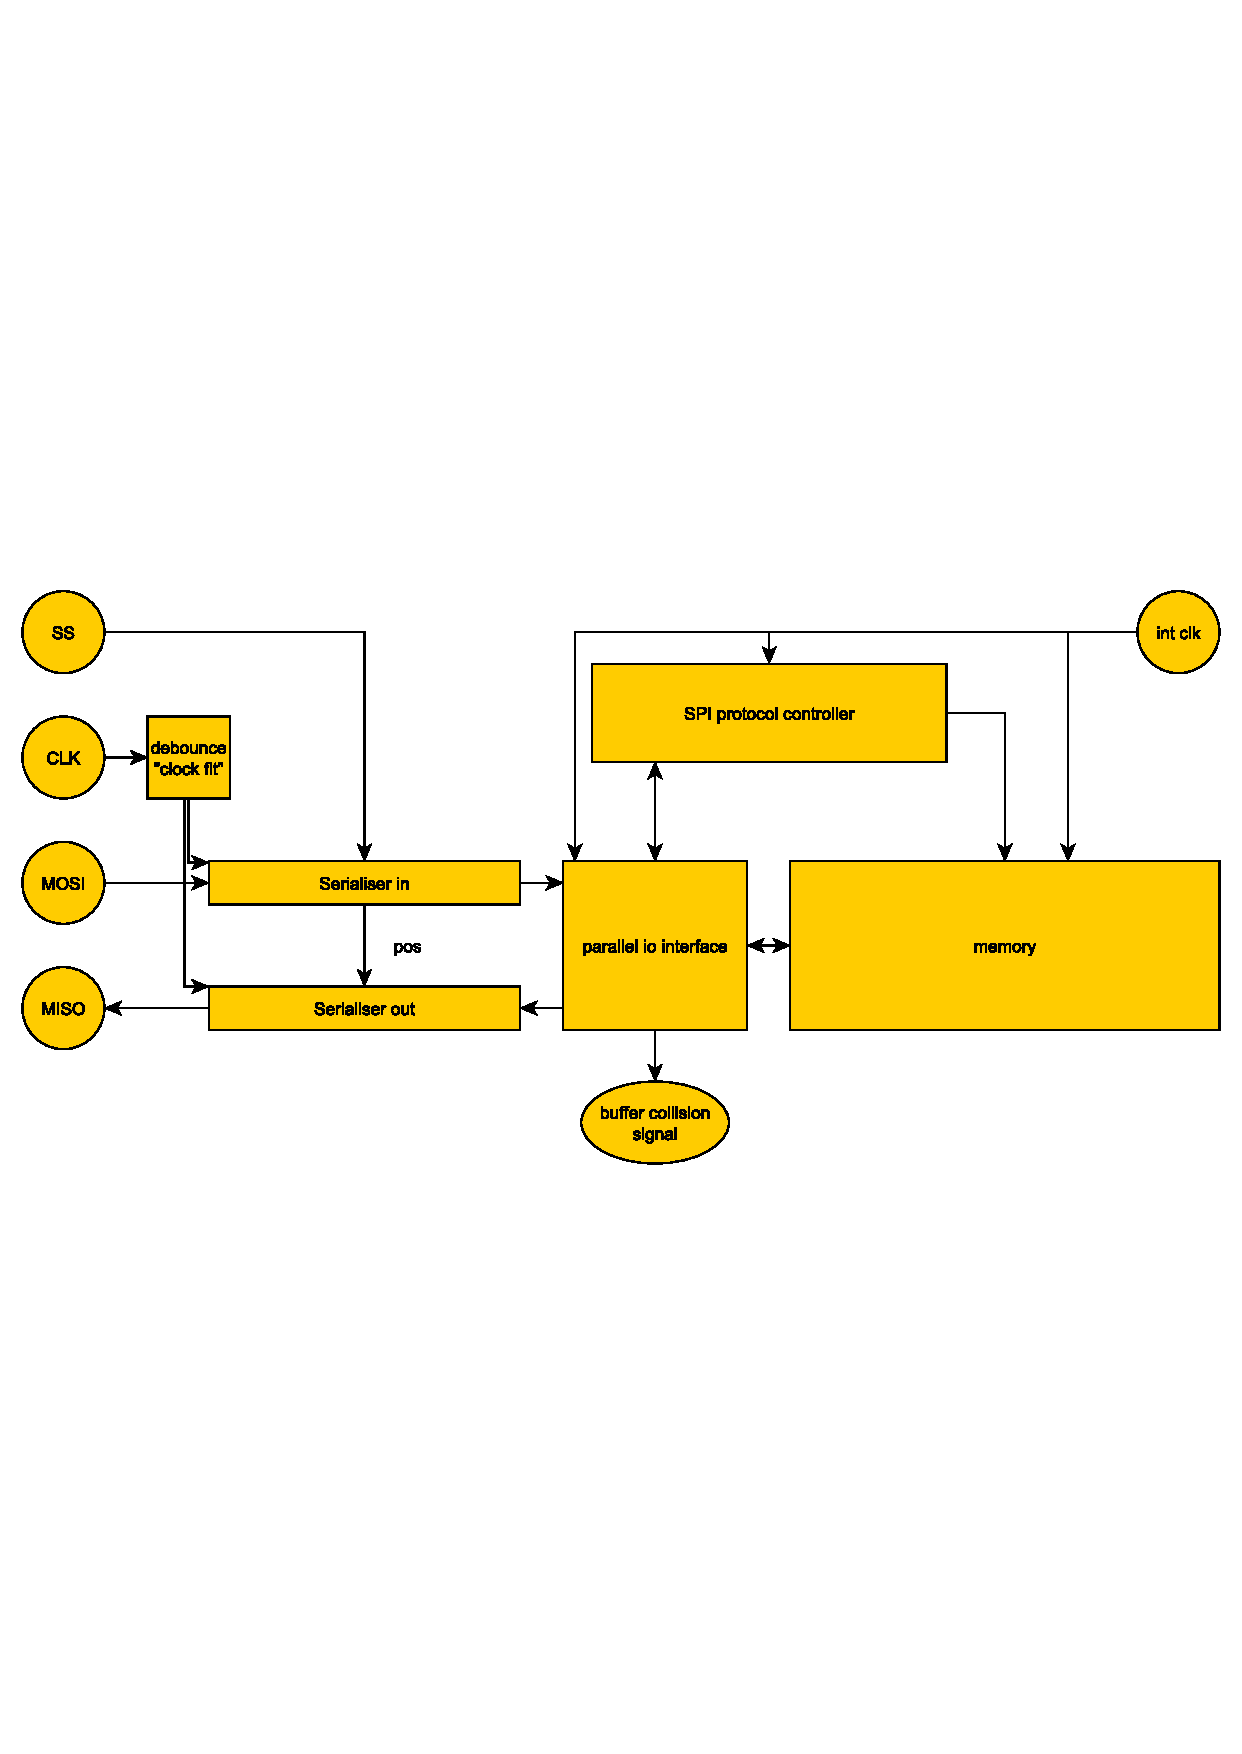
\includegraphics[width=0.96\textwidth,clip,trim=0 270 0 270]{graphics/spi_protocol_fpga_blocks_final_design.pdf}%trim=l b r t
	\caption{Blockdiagram for the SPI interface on the FPGA}
	\label{fig:spi_protocol_fpga_blocks_final_design}			% figure labels are of the form \label{fig:*}
\end{figure}

On the figure, the four SPI signals to the ARM board are present to the left, and the memory shared with the other hardware parts implemented on the FPGA to the left.

\subsection{Hardware block description}
The clock debounce process has the purpose of removing noise from the clock signal, and furthermore it can be used to change clock polarity and phase without having to change anything else in the other SPI components.

The MOSI and MISO signals are connected to the two serialiser blocks "Serialiser in" and "Serialiser out". The "Serialiser in" keeps track of the current position in the serialised data, and writes the incoming data to the respective position in the buffer. It can be seen as a demultiplexer where the debounced clock switches to next position in the buffer. When the SS signal is high, the position is always at the starting value. When transmission begins, the SS signal gets pulled low by the master, and the position starts counting accordingly to the pulses from the debounced SPI clock. 

The "Serialiser out" block can be seen as a multiplexer, where the position is fetched from the "Serialiser in" block.

The "parrallel IO interface" process presents an easy to use interface to the serialisers for internal components. It handles the serialiser buffers, and the signals involved in reading and writing from these without race conditions. The interface is made so it is possible to connect other devices then the memory block. This together with the serialisers can be considered the actual SPI hardware. 

The parallel out connections consist of these signals: \texttt{data\_out}, \texttt{data\_out\_valid}, \texttt{data\_out\_ack}\footnote{ack is short for acknowledge} and \texttt{data\_out\_buffer\_collision}. \texttt{Data\_out} and \texttt{data\_out\_ready} are output signals. When the \texttt{data\_out\_valid} is set high, the data is valid on the \texttt{data\_out} port. After the data is read, the reading device signals this by setting the \texttt{data\_out\_ack} pin to high, and the \texttt{data\_out\_valid} gets pulled low so it is ready to signal next time data is ready. If the data is not acknowledged before the next data arrives, the \texttt{data\_out\_buffer\_collision} is pulled high to warn that an internal buffer was not emptied and data was possible thrown away.

The parallel in connections works in a similar way. It consists of three signals: \texttt{data\_in}, \texttt{data\_in\_ready} and \texttt{data\_in\_ack}. When data is to be written to the SPI master, it is set on the \texttt{data\_in} port and the \texttt{data\_in\_ready} is pulled high. When the \texttt{data\_in\_ack} is set high, the data is read and the \texttt{data\_in\_ready} should be pulled low.

The SPI protocol controller has the purpose of determining how to respond to the data received on the serialser, and control the memory accordingly. The basics of the controller is a state machine which is described in \ref{spi_protocol_controller}.

As memory a true dual port ram is used, which is out-of-the-box solution from Xilinx. This RAM has two interfaces, which makes it ideal as interface between communication and other hardware block in the FPGA. The data in and data out ports are connected to the parallel interface and the write and enable signals are connected to the protocol controller. The reading and writing process of the memory module is well described in the datasheet ~\cite{XILINX_MEM}.

\subsection{SPI protocol controller}
\label{spi_protocol_controller}
The "SPI protocol controller" is a Mealey finite state machine controlling the package flow according to the protocol. It has access to read the received data from the parallel interface and sets the control signals both on the parallel interface and the memory block. When data is ready on the parallel interface it is read by the protocol controller and a decision is made about how to respond. The states of the state machine is visualised in figure \ref{fig:spi_protocol_controller_prettystates}.


\begin{figure}[htb] 
	\centering
	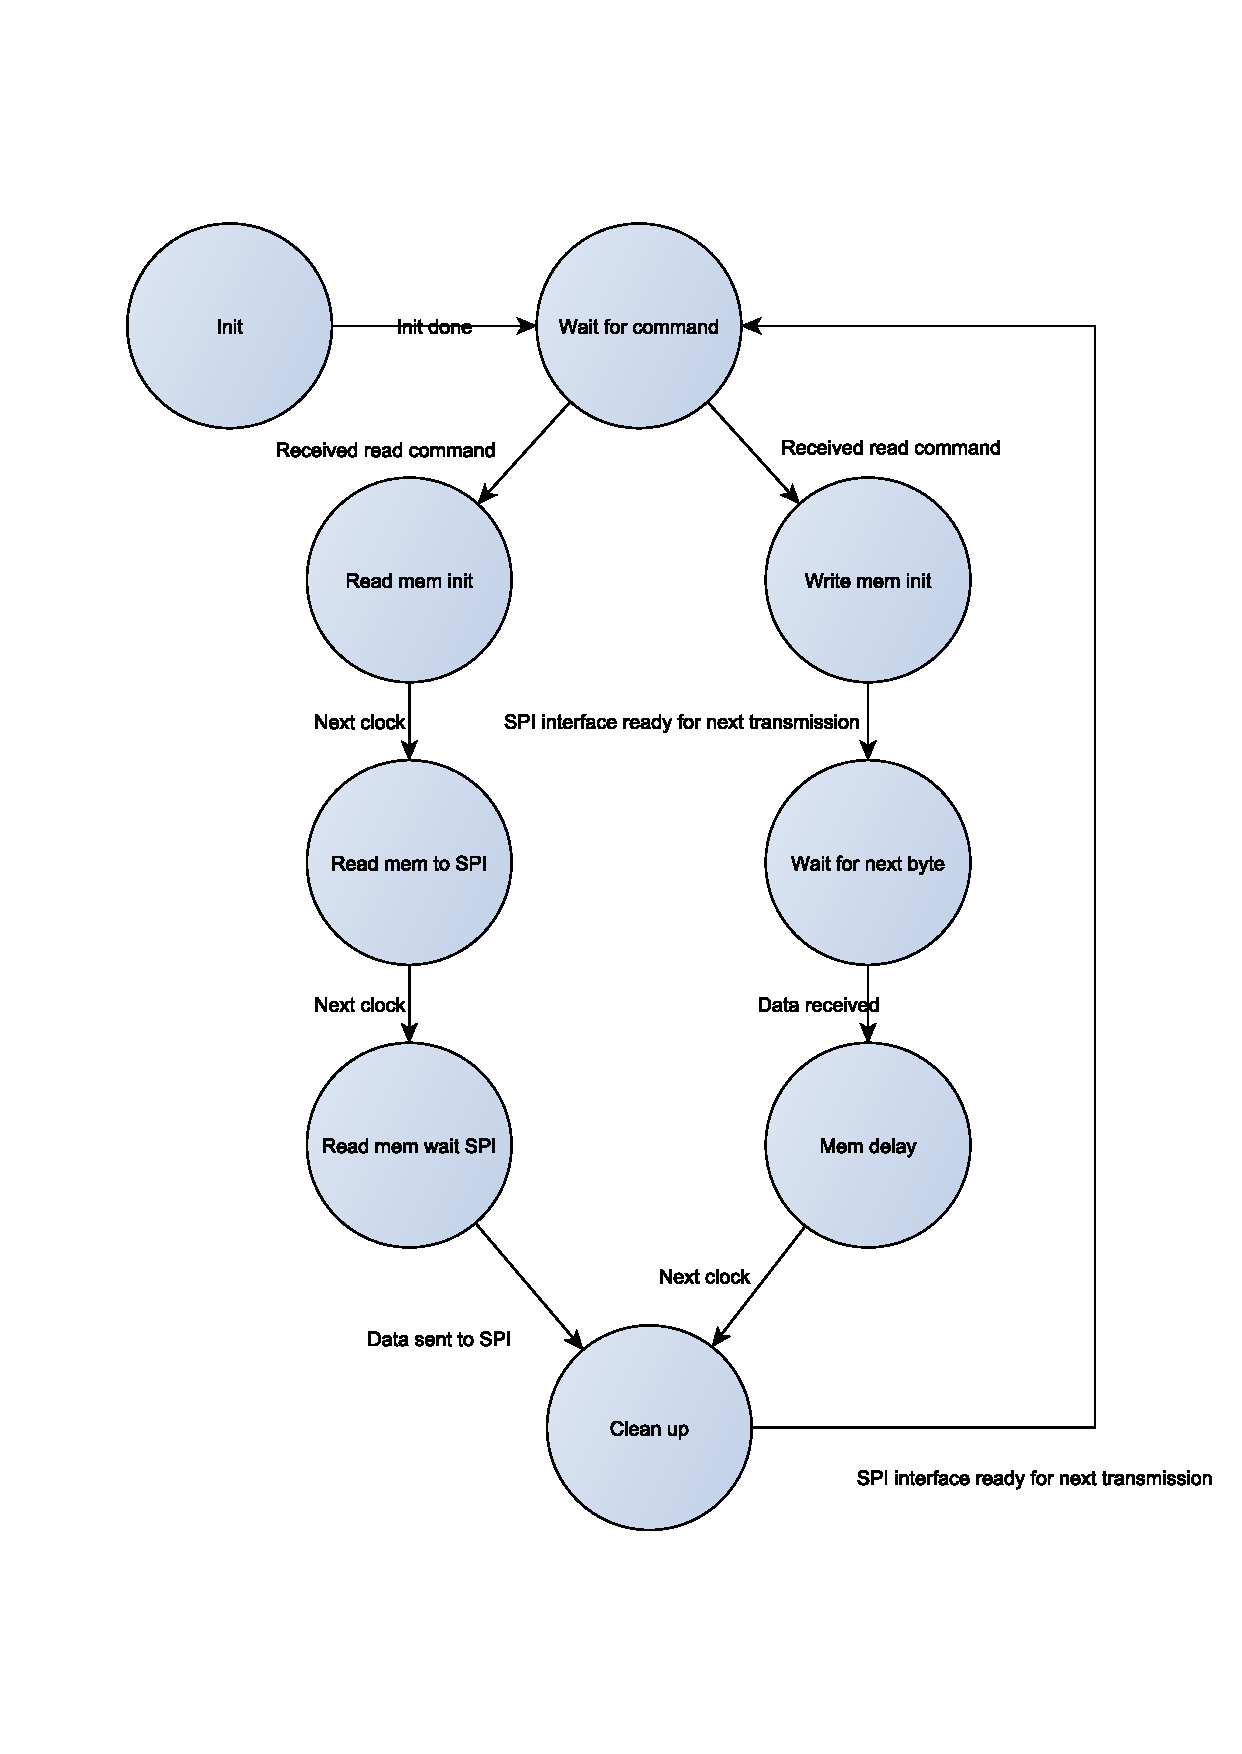
\includegraphics[scale=0.6,clip,trim=0 100 0 100]{graphics/spi_protocol_controller_prettystates.pdf} %trim=l b r t (can cut off from every side)
	\caption{State diagram for the SPI protocol controller}
	\label{fig:spi_protocol_controller_prettystates}
\end{figure}


%\begin{description}
%\item[Init] is the initial state, where it sets up the signals between the SPI and RAM to be ready. When the signals are set, it goes to "Wait for command" state.
%\end{description}

The protocol controller is started in an initial state, where it sets up the signals between the SPI and RAM to be ready. When the signals are set, it goes to a waiting mode, where it will wait for the \texttt{data\_out\_ready} to be set high. When this happens, the data/command is read and the next state depends on whether is was a read or write command.

It the received command was a read command, the next state "Read mem init" will set the requested address on the memory block, and continue to the next state "Read mem to SPI", where the \texttt{data\_out\_ready} will be set on the SPI interface. This will signal the SPI to read from mem and protocol controller will continue to the next state "Read mem wait SPI". In the "Read mem wait SPI" state, it waits for the SPI to acknowledge the data. When this is received it continues to the "Clean up" state, where waits for the SPI interface to be ready for next transmission, and returns back to the "Wait for command" state.

Another possible way through the states in the state machine, is that a write command was received in the "Wait for command" state. When the write command is received the requested write address is set on the memory block and continues to the "Write mem init" state. In the "Write mem init" state it waits for the \texttt{from\_spi\_valid} to go low, so the SPI is ready to receive next transmission. Next it goes to the "Wait for next byte" state, where it waits for the \texttt{from\_spi\_valid} to go high again, which will happen when the next transmission occur. Now it will set the "write" signal high on the memory, so the data will be saved to RAM. It then goes to the state "Mem delay" where it set the "write" signal low again, and continues to the "Clean up" state.
%Scaleability


\section{Discussion}
The protocol has been designed to carry 8 bit data sizes. This may cause a problem it a 16-bit value is transmitted, and only 8 bit has arrived when the data i read. Though if the high byte always is written first, the error is not that great. If bigger values need to be transmitted, several solutions could be considered: Increasing the size of transmitted data at once. This will be fairly easy as the ARM already supports up to max 16-bit sized data frames, and the FPGA hardware is written so it is done by changing a few parameters. Another solution would be to implement a command in the protocol for reading and writing bigger data sizes.

The protocol has been designed so the data can be abstracted away. Meaning that the protocol does not care about what data is transmitted, but just works as a carrier. If more data needs to be exchanged between the two points, it is easily done by just writing to an empty address in the memory, where the hardware is able to read it.

The SPI software was implemented with one of the main requirements being, that it should support multiple tasks using the SPI simultaneously. In the final implementation, only one task uses the SPI: The task which updates parameters to the control system. When only one task uses the SPI connection, software for handling multiple tasks is redundant and increases processing overhead. However, a watchdog software implementation\footnote{Found on the Git tree in the \texttt{watchdog\_impl} branch}, which must use SPI independently of the control parameter task, is under development. 

Using dynamic memory allocation\footnote{Memory management is discussed in detail in section \ref{sec:memoryman}} in the SPI software implementation was a deliberate choice made because of the wish to support an unknown number of user tasks. In the current state of the microcontroller application, that would not have been necessary however. The downside of using dynamically allocated memory is a slightly slower execution time and more error-prone code. The FreeRTOS kernel uses dynamically allocated memory for all of its task creation- and intertask communication API already though \cite{website:freertos-memory}, so opting for only static allocation would be meaningless unless another kernel were used; SafeRTOS for example \cite[13]{safertos}.
% REF TIL TEST

%
%\subsection{Test}
%Experiments chapter.
%
%
%
%\subsection{Discussion?}
%Pros/cons\\
%Possible optimization\\
%Is it inefficient?\\
%Overhead linearly proportional with amounts transmitted/received?\\
%Tasks transmission priority is decided by the order in which they use \texttt{spi\_register\_task()}

The implementation process of the SPI on the FPGA saved a lot of time. The idea of first having a working model in the simulation environment and then build to the platform, spared a lot of on-hardware debugging and synthesising time. The testing was done with a device known to work with SPI, enabling the FPGA SPI part to be tested before it was fully implemented on the ARM.

On the FPGA, a 32byte dual port RAM has been used as interface between SPI and motor controller. This has been a great advantage during design and testing, as the parts where able to be tested separately and put together afterwards.

The protocol and FPGA hardware was tested for reliability, which are described in \ref{sec:spi_rel_test}. In the test it is concluded that the protocol and hardware can transmit without errors with cables lengths up to 25cm.



\section{Conclusion}
A protocol for communication between the ARM and FPGA has been designed. The protocol has been implemented on the ARM as software and hardware on the FPGA. Test shows that the protocol and the implementation can work with a error rate of 0\% in a normal environment with short cables.


% Block overview / hardware planning
% Block description
% Testbench
